%!TEX root = bachelor.tex
\chapter{Theoretische Grundlagen}
\label{ch:theory}

In diesem Kapitel werden einige Grundlagen für die folgende Kapitel eingeführt. 


Wir benutzen ein linkshändiges Koordinatensystem.



\section{Kegel}
\label{s:cone}

\begin{definition}[Kegel]
	Ein Kegel ist ein geometrischer Körper, der durch eine beliebige Grundfläche, sowie einen Punkt definiert wird.
	Ein Kegel mit Kreis als Grundfläche wird als Kreiskegel bezeichnet. Liegt die Kegelspitze auf einer Geraden durch die Normale der Grundebene, bezeichnen wir den Kegel als gerade.
\end{definition}

In der weiteren Arbeit betrachten wir nur gerade Kreiskegel.
$S$ bezeichne hierbei die Seitenhöhe und ist definiert durch $S = \sqrt{H^2 + R^2}$ (siehe Abbildung \ref{fig:cone}).

\begin{figure}[!htb]
	\centering
	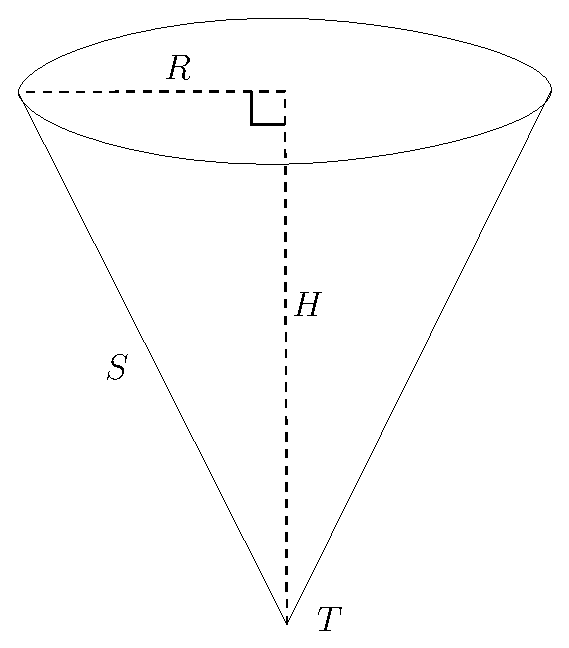
\includegraphics[scale=.5]{images/fullCone.eps}
	\caption{Gerader Kreiskegel}
	\label{fig:cone}
\end{figure}

Ein Kegel mit Spitze $T(0,0,0)$, Radius $R$ und Höhe $H$ kann parametrisch beschrieben werden als:
\begin{equation}
\begin{aligned}
x &= \frac{u}{h} R~cos \theta \\
y &= u \\
z &= \frac{u}{h} R~sin \theta
\end{aligned}
\end{equation}
mit $u\in [0, H]$ und $\theta \in [0, 2\pi)$ 


\begin{definition}[Kegelstumpf und Ergänzungskegel]
	Ein Kegelstumpf entsteht als Schnitt eines geraden Kreiskegels mit einer zur Grundfläche parallelen Ebene (siehe Abbildung \ref{fig:coneWithFrustum}). Das Stück von Grundfläche zur Schnittfläche nennen wir Kegelstumpf. Die Differenz zum eigentlichen Kegel wird als Ergänzungskegel bezeichnet. 
	
	$H, R, S$ bleiben die Angaben des gesamten Kegels. Hinzu kommen $h,r,s$ als Angaben des Ergänzungskegels. Die Höhe, sowie die Seitenhöhe des Kegelstumpfs werden durch die Differenzen $\Delta S = S - s,~ \Delta H = H-h$ charakterisiert (siehe Abbildung \ref{fig:coneFrustum}).
\end{definition}

\begin{figure}[!htb]
	\centering
	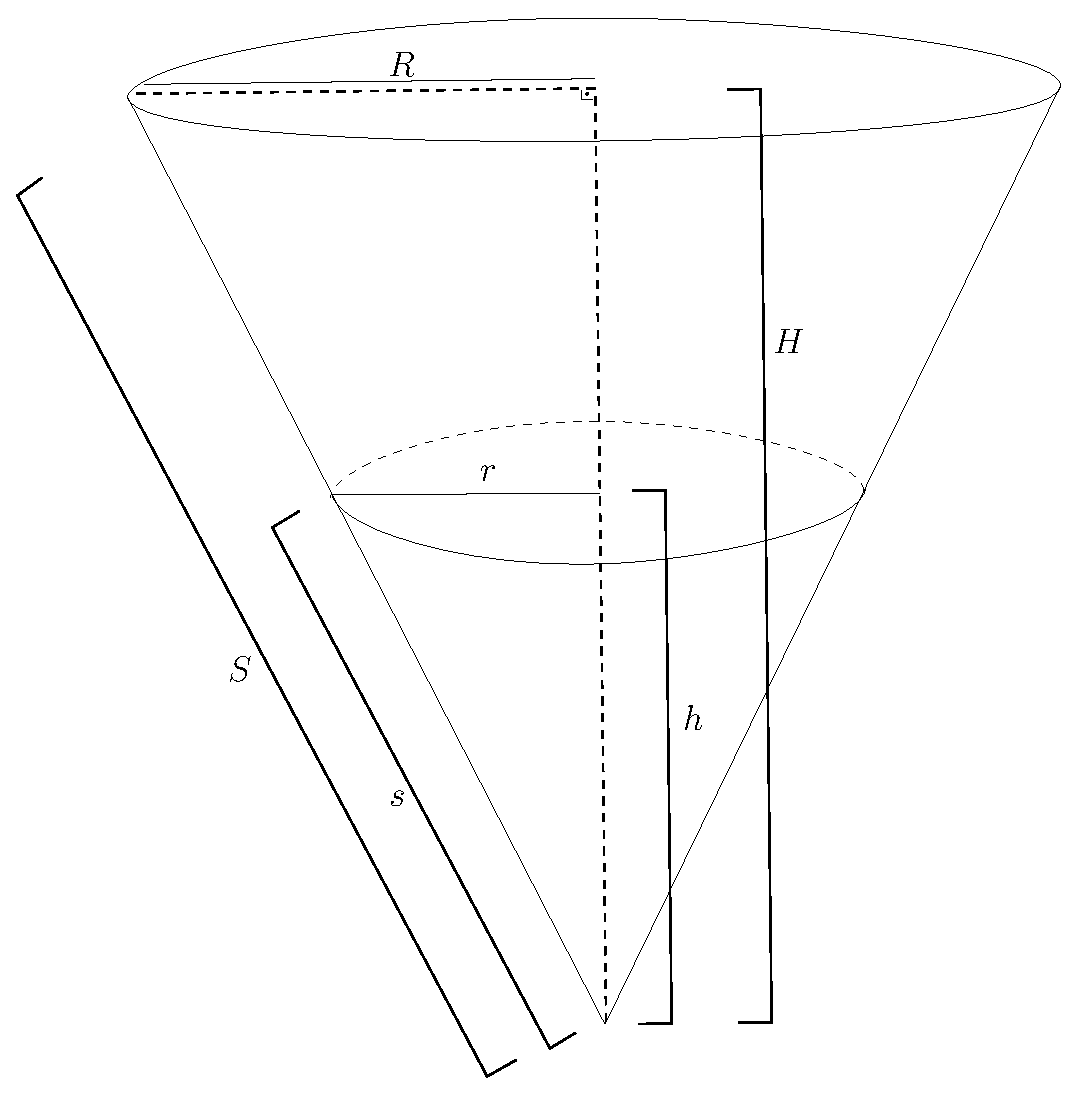
\includegraphics[scale=.5]{images/fullCone3.eps}
	\caption{Kegelstumpf und Ergänzungskegel}
	\label{fig:coneWithFrustum}
\end{figure}

\begin{figure}[!htb]
	\centering
	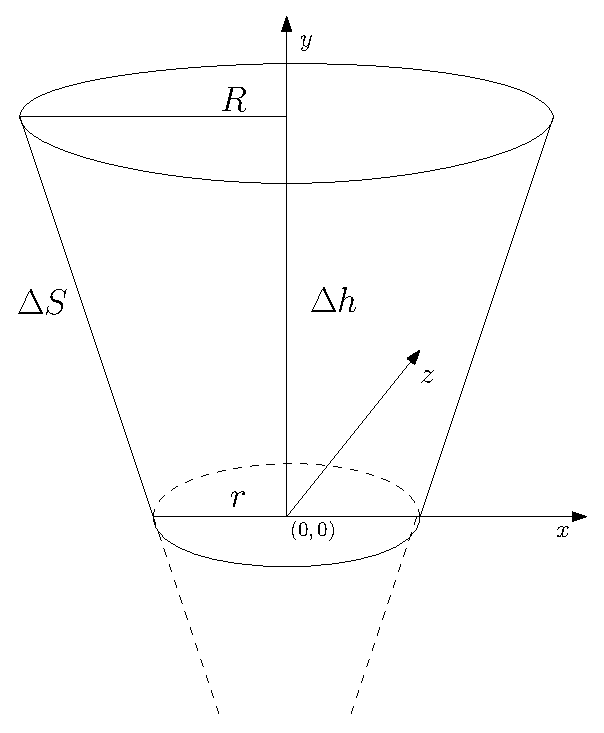
\includegraphics[scale=.7]{images/coneFrustum.eps}
	\caption{Kegelstumpf}
	\label{fig:coneFrustum}
\end{figure}

Analog zum Kreiskegel definieren wir einen Kegelstumpf durch folgende Parametrisierung: 
\begin{equation} \label{eq:paramFrustum}
\begin{aligned}
x &= (r + \frac{u}{\Delta H} (R - r))~cos \theta \\
y &= u \\
z &= (r + \frac{u}{\Delta H} (R - r))~sin \theta
\end{aligned}
\end{equation}
mit $u\in [0, \Delta H]$ und $\theta \in [0, 2\pi)$


\begin{figure}[!htb]
	\centering
	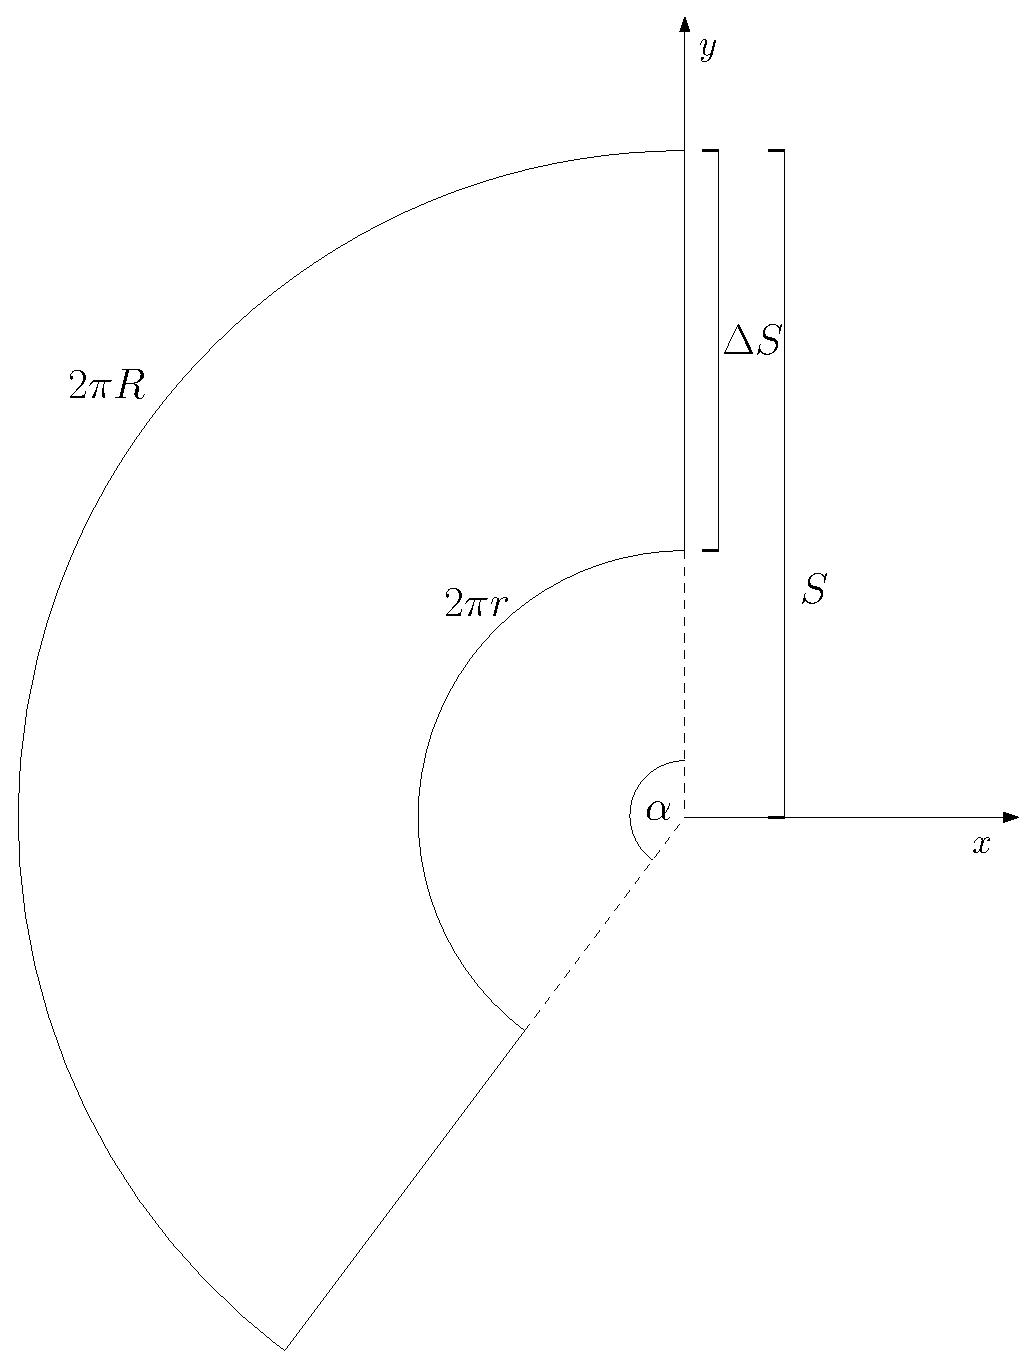
\includegraphics[scale=.4]{images/coneLateral.eps}
	\caption{Kegelmantelfläche}
	\label{fig:coneLateral}
\end{figure}

Die Mantefläche des Kegelstumpfes aus Abbildung \ref{fig:coneLateral} kann dann parametrisch beschrieben werden als:
\begin{equation} \label{eq:paramLateral}
\begin{aligned}
x &= -(s + \frac{u}{\Delta H}(S-s)) ~sin \phi \\
y &= (s + \frac{u}{\Delta H} (S-s)) ~cos \phi
\end{aligned}
\end{equation}
mit  $u\in [0, \Delta H]$ und $\phi \in [0, \alpha] \subseteq [0, 2\pi]$ mit $\alpha S = 2\pi R \implies \alpha = 2\pi\frac{R}{S}$

\bigskip

Ein Punkt auf der Oberfläche des Kegelstumpfs kann eindeutig einem Punkt auf der Mantelfläche (und umgekehrt) zugeordnet werden. Dazu konstruieren wir folgende Abbildung und ihr Inverses:

Sei ein Punkt $C(x,y,z)$ auf der Oberfläche des Kegelstumpfs gegeben. Wir wissen aus der parametrischen Form \ref{eq:paramFrustum}, dass $C$ die Form
\[
C(x,y,z) = (r + \frac{u}{\Delta H} (R - r))~cos \theta, u, (r + \frac{u}{\Delta H} (R - r))~sin \theta
\]  für ein $u\in [0, \Delta H]$ und $\theta \in [0, 2\pi)$ besitzt. 

Aus der $y$-Koordinate kann man als die Höhe ablesen und somit den Radius in der Mantelfläche als lineare Interpolation zwischen $s$ und $S$ bestimmen (siehe Abbildung \ref{fig:mapToLateralS}). Wir definieren uns hierfür eine Hilfsfunktion 
\begin{equation} \label{eq:Sigma}
	\Sigma(y) := s + \frac{y}{\Delta H} (S-s)
\end{equation}


\begin{figure}[!htb]
	\centering
	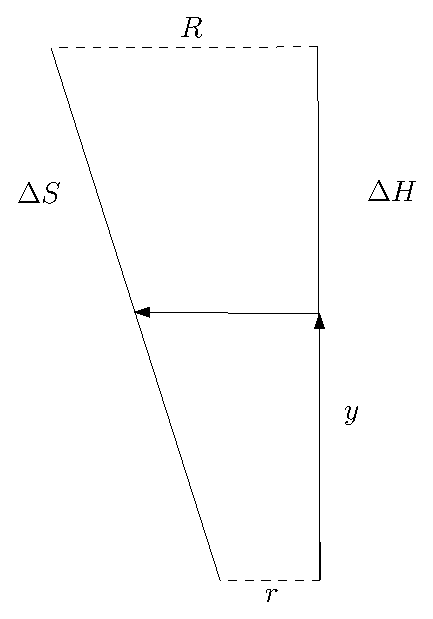
\includegraphics[scale=.7]{images/mapToLateralS.eps}
	\caption{Abbildung der Kegelstumpfhöhe auf die Seitenhöhe}
	\label{fig:mapToLateralS}
\end{figure}

Da $R, r, \Delta H$  und nun auch die Höhe bekannt sind, kann man den Winkel $\theta$ im Kegelstumpf einfach ausrechnen. Anschließend muss dieser noch mit  $\frac{R}{S}$ multipliziert werden um ihn auf $[0, \alpha]$ zu skalieren (siehe \ref{eq:paramLateral}).  Auch hierfür definieren wir eine Hilfsfunktion:
\begin{equation*}
\Phi(x,y,z) := \frac{R}{S} \atant\left(\frac{z}{r + \frac{y}{\Delta h} (R - r)}, \frac{x}{r + \frac{y}{\delta H} (R - r)}\right),
\end{equation*}

wobei wir $\atant$ benutzen um den Winkel im richtigen Quadranten, also in $[0, 2\pi)$, bestimmen zu können. 

Mit diesen beiden Hilfsfunktionen und \ref{eq:paramLateral} ergibt sich insgesamt:
\begin{equation}\label{eq:coneToLateral}
\begin{aligned}
\Psi \colon [r,R] \times [0, \Delta H] \times [r,R] &\to [s,S] \times [s,S]\\
\begin{pmatrix}
x \\ y \\ z
\end{pmatrix}  &\mapsto
\begin{pmatrix}
-\Sigma(y)\sin \Phi(x,y,z)\\
 \Sigma(y)\cos\Phi(x,y,z)
\end{pmatrix}
\end{aligned}
\end{equation}

Analog lässt die sich Umkehrabbildung konstruieren:

Sei ein Punkt $L(x,y)$ auf der Mantelfläche des Kegelstumpfs gegeben. Aus der parametrischen Form \ref{eq:paramLateral} ergibt sich

\[
L(x,y) = (-(s + \frac{u}{\Delta H}(S-s)) ~sin \phi, (s + \frac{u}{\Delta H} (S-s)) ~cos \phi)
\]

für ein passendes $u\in [0, \Delta H]$ und $\phi \in [0, \alpha] \subseteq  [0, 2\pi]$.

Da $L(x,y)$ in Polarkoordinaten gegeben ist, lässt sich der Radius durch $\sqrt{x^2+y^2}$ bestimmen. Wir können den Winkel $\phi$ mit inverser Skalierung also analog durch folgende Hilfsfunktion bestimmen:

\begin{equation*}
\Theta(x,y) := \frac{S}{R} \atant\left(\frac{x}{-\sqrt{x^2+y^2}}, \frac{z}{\sqrt{x^2+y^2}}\right)
\end{equation*}

Die Höhe  im Kegel und somit der Radius lässt sich nun gewissermaßen als Umkehrabbildung zu \ref{eq:Sigma} bestimmen:
\begin{equation*}
\mathrm{H}(x,y) := \frac{\left(\sqrt{x^2+y^2}\right) - s}{S - s}\Delta H
\end{equation*}

Insgesamt ergibt sich:
\begin{equation}\label{eq:LateralToCone}
\begin{aligned}
\Psi^{-1} \colon  [s,S]x[s,S] &\to [r,R] \times [0, \Delta H] \times [r,R]\\
\begin{pmatrix}
x \\ y
\end{pmatrix} &\mapsto
\begin{pmatrix}
\left( r + \frac{\mathrm{H}(x,y)}{\Delta H} (R - r)\right)\cos\left(\Theta(x,y) \right) \\
\mathrm{H}(x,y)\\
\left( r + \frac{\mathrm{H}(x,y)}{\Delta H} (R - r)\right)\sin\left(\Theta(x,y) \right)
\end{pmatrix}
\end{aligned}
\end{equation}


\section{Lineares Ausgleichsproblem}
\label{s:LSQ}
Gegeben seien $m$ Messdaten $(x_1,y_1),\dotsc,(x_m,y_m)$, sowie eine lineare Funktion $\varphi(x) = \sum_{i = 1}^{n}c_i\varphi_i(x)$ in $x$ mit $c_1,\dotsc,c_n\in\mathbb{R}$, $n\leq m$ und $n,m\in\mathbb{N}$. 

Gesucht ist eine Lösung der $c_i$ welche die mittlere Abweichung, also 

\[
\Delta_2 = \min_{c_1,\dotsc,c_n\in\mathbb{R}} \left(\sum_{j=1}^{m}\left(y_j - \varphi(x_j)\right)^2\right) = \min_{c_1,\dotsc,c_n\in\mathbb{R}} \left(\sum_{j=1}^{m}\left(\sum_{i=1}^{n}y_j-\left(c_i\varphi_i(x_j)\right)\right)^2\right)
\]

minimiert \cite{Stoer2007}.

Diese Problem wird als lineares Ausgleichsproblem oder aber auch als Methode der kleinsten Quadrate bezeichnet und lässt sich auch wie folgt formulieren:

\[
\min_{c\in\mathbb{R}^n} ||y - Ac||_2,
\]

mit 
\[
\begin{aligned}
c &= (c_1,\dotsc,c_n)^T\in\mathbb{R}^n \\
x &= (x_1,\dotsc,x_m)^T\in\mathbb{R}^m \\
y &= (y_1,\dotsc,y_m)^T\in\mathbb{R}^m \\
A &= (a_{ij})\in\mathbb{R}^{m\times n}\quad\text{mit}\quad a_{ij} = \varphi_i(x_j)
\end{aligned}
\]

Das Problem lässt sich auch mit Hilfe der äquivalenten sogenannten Normalengleichung
\begin{equation*}
	(A^TA)c = A^Ty
\end{equation*}

lösen, wobei mindestens eine Lösung existiert und die Lösung mit kleinster 2-Norm eindeutig ist. 

Gilt darüber hinaus $\text{rang}\left(A\right) = n$ so ist $A^TA$ invertierbar und es gilt 

\begin{equation}\label{eq:normaleq}
c = \underbrace{(A^TA)^{-1}A^T}_{A^+}y
\end{equation}

und c ist die eindeutige Lösung mit kleinster 2-Norm.

$A^+$ bezeichnet man auch als Pseudoinverse von $A$ und lässt sich durch eine Singulärwertzerlegung (SVD) bestimmen \cite{Stoer2011}. Die Matrizen $A\in\mathbb{R}^{m\times n}$ und $A^+\in\mathbb{R}^{n\times m}$ können geschrieben werden als:

\[
\begin{aligned}
A &= U\Sigma V^T \\
A^+ &= V\Sigma^+U^T
\end{aligned}
\]

mit orthogonalen Matrizen $U\in\mathbb{R}^{m\times m}$ und $V\in\mathbb{R}^{n\times n}$ und einer Diagonalmatrix $\Sigma\in\mathbb{R}^{m\times n}$ mit den absteigend sortierten Singulärwerten auf der Diagonale (aufgefüllt mit Nullen), sowie $\Sigma^+\in\mathbb{R}^{n\times m}$ mit den jeweiligen reziproken Singulärwerten.


Die Lösung des Ausgleichsproblems kann also mittels SVD angeben werden als:
\[
c = V\Sigma^+U^Ty
\]



\section{Kamerakalibrierung und projektive Geometrie}
\label{s:calib}

\begin{definition}
	Kamerakalibrierung ist ein Verfahren, bei dem die interne Kamerageometrie und optischen Eigenschaften (intrinische Parameter) 
	und/oder die 3D-Position und Orientierung der Bildebene relativ zu einem Weltkoordinatensystem (extrinische Parameter) bestimmt werden \cite{Tsai1987}.
\end{definition}
\bigskip
Um die Parameter einer Kamera korrekt beschreiben zu können, ist ein Kameramodell notwendig. Das wohl bekannteste Kameramodell ist das Lochkamera-Modell. Die Lichtstrahlen der Szene gelangen dabei durch eine kleine Öffnung in die Kamera (siehe dazu Abbildung \ref{fig:pinhole}).
\begin{figure}[!htb]
	\centering
	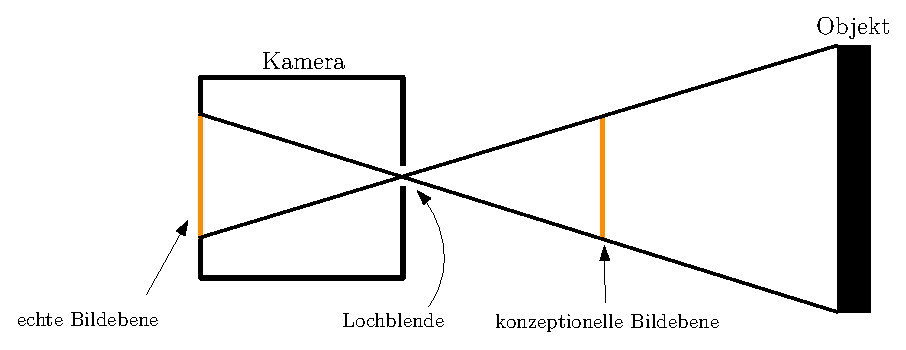
\includegraphics[scale=.8]{images/pinhole2.eps}
	\caption{Lochkameramodell}
	\label{fig:pinhole}
\end{figure}

Das Bild das an der Rückseite der Kamera entsteht ist dabei um 180° gedreht. Damit man diese Rotation nicht betrachten muss, kann man die Bildebene virtuell vor die Lochblende setzen. Da sich der Abstand zur Blende nicht ändert, ändern sich, außer der ersparten Rotation, auch die optischen Eigenschaften nicht.

Kamerakalibrierung wird benötigt, um eine Beziehung zwischen Punkten in 3D im Weltkoordinatensystem und den Punkten auf der Bildebene herzustellen. Konkret suchen wir eine projektive Abbildung

\begin{equation}
	\begin{pmatrix}
	wu \\wv \\w 
	\end{pmatrix} = 
		\underbrace{\begin{pmatrix}
		a_{11} & a_{12} & a_{13} & a_{14} \\
		a_{21} & a_{22} & a_{23} & a_{24} \\
		a_{31} & a_{32} & a_{33} & a_{34} 
		\end{pmatrix}}_{=:A}	\begin{pmatrix}
		x \\y \\z \\ 1 
		\end{pmatrix},
\end{equation}


die einen Punkt $P=(x,y,z)$ in homogenen Koordinaten $\tilde P = (x,y,z,1)$ auf einen Punkt $\tilde C = (wu,wv, w)$ beziehungsweise nach der perspektivischen Division $C = (u,v)$ auf die Bildebene abbildet, wobei die $a_{ij}$ von den intrinsischen und extrinsischen Parametern der Kamera abhängen \cite{Heikkila1997}.

Man kann leicht zeigen, dass für $A$ gilt
\[
A = \lambda \cdot
\begin{pmatrix}
1 & 0 & u_0\\
0 & 1 & v_0\\
0 & 0 & 1 
\end{pmatrix}
\begin{pmatrix}
f & 0 & 0\\
0 & f & 0\\
0 & 0 & 1 
\end{pmatrix} 
\left(\begin{array}{ccc}
R &  T\\
0 & 1 
\end{array}\right) = \lambda\underbrace{\begin{pmatrix}
f & 0 & u_0\\
0 & f & v_0\\
0 & 0 & 1 
\end{pmatrix}}_{=:V}
\left(\begin{BMAT}(e)[1pt]{ccc|c}{ccc|c}
& & & \\
& \text{\large R}& & \text{\large T} \\
& &  & \\
0 & 0 & 0 & 1
\end{BMAT}\right),
\]

wobei $\lambda$ ein beliebiger Skalierungsfaktor ist. $V$ beschreibt die intrinsischen und $R$ und $T$ die extrinsischen Parameter (siehe \cite{Heikkila1997}). $f$ ist hierbei die Brennweite; $u_0$ und $v_0$ die Bildmitte.

%Zunächst wird also das Weltkoordinatensystem wie in Abbildung \ref{fig:extrinsic} mit einer Rotation und einer Translation in das Kamerakoordinatensystem überführt. Anschließend wird 
 
 Zu gegebenen Punktenpaaren $(x_k,y_k), k = 1,\dotsc,m$ kann diese Matrix wie folgt gelöst werden:
 
 \begin{equation*}
 \begin{aligned}
 u_k &= \frac{a_{11} x_k +a_{12}y_k + a_{13}z_k + a_{14}}{a_{31} x_k +a_{32}y_k + a_{33}z_k + a_{34}} \\
 v_k &= \frac{a_{21} x_k +a_{22}y_k + a_{23}z_k + a_{24}}{a_{31} x_k +a_{32}y_k + a_{33}z_k + a_{34}}
 \end{aligned}
 \end{equation*}
 
 \setcounter{MaxMatrixCols}{20}
\begin{equation}\label{eq:DLT}
\underbrace{\begin{pmatrix}
x_1 & y_1 & z_1 & 1 & 0 & 0 & 0 & 0 & -u_1 x_1 & -u_1 y_1 & -u_1z_1 \\
0 & 0 & 0 & 0 & x_1 & y_1 & z_1 & 1 & -v_1x_1 & -v_1y_1 & -v_1z_1 \\
\vdots & \vdots & \vdots & \vdots & \vdots & \vdots & \vdots & \vdots & \vdots & \vdots & \vdots\\
x_m & y_m & z_m & 1 & 0 & 0 & 0 & 0 & -u_m x_m & -u_m y_m & -u_m z_m \\
0 & 0 & 0 & 0 & x_m & y_m & z_m & 1 & -v_mx_m & -v_my_m & -v_mz_m
\end{pmatrix}}_{=:M}
\begin{pmatrix}
a_{11} \\ a_{12} \\ a_{13} \\ a_{14} \\ a_{21} \\ a_{22} \\ a_{23} \\ a_{24} \\ a_{31} \\ a_{32} \\ a_{33}
\end{pmatrix} = 
\begin{pmatrix}
u_1 \\ v_1 \\ \vdots \\ u_m \\ v_m
\end{pmatrix},
\end{equation}

wobei $a_{34}$ auf eins skaliert wird.  Es handelt sich hierbei um ein überbestimmtes lineares Gleichungssystem, was mittels der Methode der kleinsten Quadrate (siehe Kapitel \ref{s:LSQ}) gelöst werden kann. 
Diese Verfahren wird auch als \textit{Direct Linear Transformation}(DLT) bezeichnet.
 
Das beschriebene Verfahren vernachlässigt dabei Linsenverzerrungen. Solche Verzerrungen entstehen entweder als Produktionsfehler günstiger Linsen, oder bewusst beispielsweise bei Weitwinkelkameras. Verzerrungen können in der Regel nicht linear modelliert werden. Der Ansatz über DLT funktioniert hier dementsprechend nicht. 
 
 \todo{hier muss noch was getan werden}DLT vernachlässigt alle Verzerrungen. Um diese zu kompensieren benutze die 4 schritte von tsai
 

Die vier Schritt der Kamerakalibrierung sind nach Tsai\cite{Tsai1987}:
\begin{enumerate}
	\item Rotation und Translation des Weltkoordinatensystems, um es in das Bildkoordinatensystem zu überführen.
	\item Perspektivische Division und Skalierung mit der Brennweite
	\item Bestimmen der Verzerrungskoeffiezienten $\kappa_1$ und $\kappa_2$
\end{enumerate}

\begin{figure}[!htb]
	\centering
	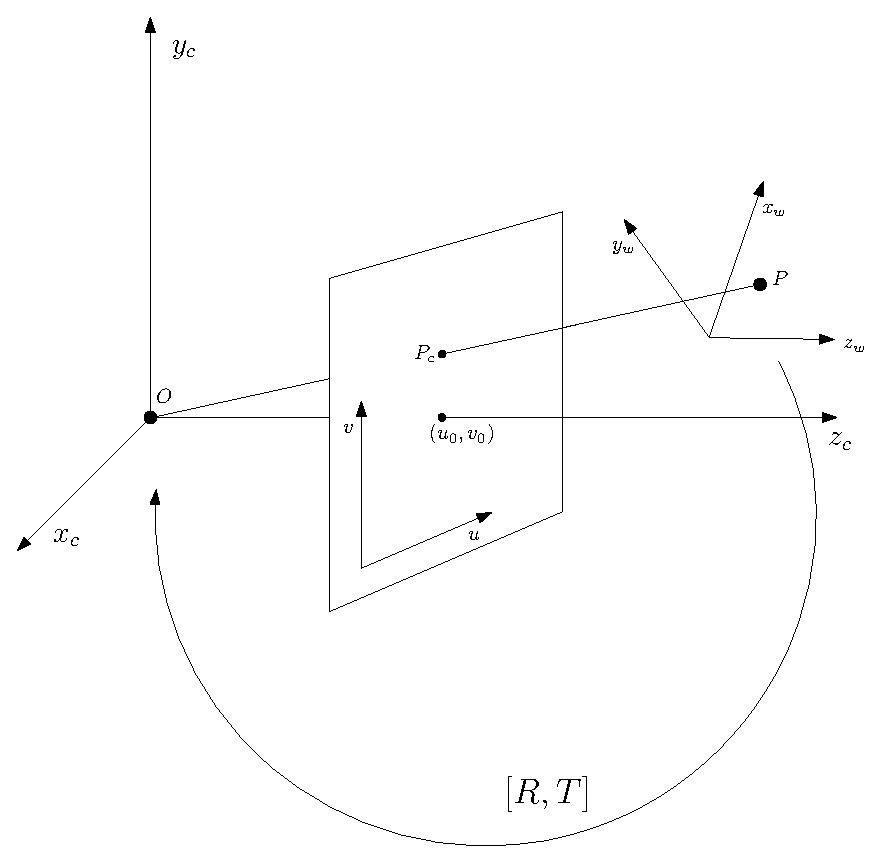
\includegraphics[scale=.8]{images/pinhole.eps}
	\caption{Projektion eines Punktes $P$ im Weltkoordinatensystem $(x_w, y_w, z_w)$ auf die Bildebene im Kamerakoordinatensystem  $(x_c, y_c, z_c)$}
	\label{fig:extrinsic}
\end{figure}



Selfcalibrating vs bla bla




\section{Blob-Detektor}
\label{s:blob}
\begin{definition}[Blob]\label{def:blob}
	Ein Blob ist eine glatte zusammenhängende Region in einem Bild, die sich farblich von ihrer Umgebung abhebt \cite{Lindeberg1993}.
\end{definition}

Ein Blob-Detektor ist also ein Verfahren zum Detektieren solcher Blobs. Die gefunden Blobs können anschließend nach verschiedenen Kriterien, wie Größe, Farbe, Konvexität oder Rundheit gefiltert werden. 

\section{Canny}
\label{s:canny}
Der Canny-Algorithmus\cite{Canny1986} ist ein Verfahren zur Kantendetektion. Im Gegensatz zu anderen Verfahren wie Sobel, oder Prewitt, versucht Canny die Fehlerrate der Kantendetektion minimal zu halten. 
Es sollten nicht mehr Kanten zurückgegeben werden, als auf dem Bild zu sehen und es sollten auch keine Kanten übersehen werden. Darüber hinaus markiert Canny die Kanten möglichst exakt, minimiert also die Distanz eines markierten Punktes zur eigentlichen Kante. Zuletzt gewährleistet Canny außerdem die Eindeutigkeit einer Kante. Das bedeutet, dass eine Kante nicht mehrmals markiert wird.

\section{Hough-Transformation}
\label{s:hough}
Hough-Transformation ist ein Verfahren zur Detektion von beliebigen parametrisierbaren Konturen. In dieser Arbeit werden Hough-Transforamtionen benutzt um Geraden zu detektieren. 

Eine beliebige zweidimensionale Gerade kann in Polarkoordinaten folgendermaßen implizit ausgedrückt werden:

\begin{equation}\label{eq:HoughLines}
x\cos\phi + y\sin\phi - d = 0,
\end{equation}

wobei $\phi \in [0,2\pi)$ der Winkel der Geraden mit der $X$-Achse und $d \geq 0$ der Radius, also der euklidische Abstand der Geraden zum Ursprung des Koordinatensystems ist.

Eine Gerade wird somit als ein Punkt $(d,\phi)$ in den Parameterraum (auch Hough-Raum) abgebildet. 

Um eine Gerade eindeutig zu definieren benötigt man, wie auch bei der klassischen Defintionen $y = mx + b$, zwei Punkte. Nimmt man nur einen, so lässt sich jedoch die Auswahl von $\phi$ und $d$ einschränken. Hat man beispielsweise einen Punkt $(x_k,y_k)$ gegeben so lässt sich die Gleichung \ref{eq:HoughLines} nach $d$ umstellen und man erhält eine sinusförmige Funktion in Abhängigkeit von $\phi$. 

Um beliebige Geraden detektieren zu können, werden $\phi$ und $d$ passen diskretisiert:
\begin{equation*}
	\begin{aligned}
		\phi_i &= \phi_{min} + \frac{i}{n} \cdot (\phi_{max} - \phi_{min}) \quad&\forall &i\in [0,n]\\
		d_j &= d_{min} + \frac{j}{m} \cdot  (d_{max} - d_{min}) &\forall &j\in [0,m]
	\end{aligned}
\end{equation*}

Es wird nun ein Akkumulator $\mathcal{H}(\phi, d)$ für alle $\phi_i$ und $d_j$ auf null gesetzt.

Als Nächstes wird ein Kantentbild mittels Canny erzeugt und jene Pixel $(x_k,y_k)$ betrachtet, die nicht null sind.
Zu einen gegebenen Pixel wir nun für alle diskreten Winkel $\phi_i$ ein $d_i$ ausgerechnet und entsprechend im Akkumulator  $\mathcal{H}$ der Wert an der Stelle $(\phi_i, d_i)$ erhöht. 
Am Ende des Verfahrens such man im Akkumulator nach Häufungspunkten. Jeder Häufungspunkt steht dort für eine Gerade. 


\section{RANSAC}
\label{s:ransac}
\textit{Random Sample Consensus} (RANSAC) \cite{Fischler1981} ist ein nicht-deterministisches robustes Verfahren zur Parameterschätzung eines Modells bei einer, möglicherweise durch starke Ausreißer, gestörten Messreihe. 
Im Gegensatz zu Verfahren, wie der Methode der kleinsten Quadrate, die versuchen eine optimale Lösung für alle Messdaten zu bestimmen, nutzt RANSAC nur eine Teilmenge der Messreihe. 

RANSAC wählt aus der Menge der Messdaten wiederholt zufällig die minimale Anzahl Messdaten aus, die nötig sind um das Modell eindeutig zu beschreiben und prüft dann, wie gut das geschätzte Modell die restlichen Messdaten beschreibt. 
Die Güte des Modells wird im Allgemeinen durch ein Distanzmaß, wie zum Beispiel der euklidische Abstand, berechnet. 
Hat ein Messdatum eine vorher definierte Maximaldistanz zum geschätzten Modell nicht überschritten, wird es ins sogenannte Consensus Set des Modells aufgenommen. 
Das Modell mit dem größten Consensus Set wird schließlich ausgewählt. 

Die Anzahl der Iterationen, die mindestens notwendig sind, um mit einer Wahrscheinlichkeit von $p \in [0,1)$, bei einem relativen Ausreißeranteil von $\epsilon \in[0,1)$ und einer Anzahl von $k$ Daten, um das Modell eindeutig zu beschreiben, mindestens einmal eine ausreißerfreie Teilmenge der Messreihe zu erhalten, lässt sich berechnen mit:

\begin{equation}
\frac{\log{\left(1-p\right)}}{\log{\left(1-\left(1-\epsilon\right)^k\right)}}
\end{equation}


\section{Ellipsen}
\label{s:ellipse}
\subsection{allgemein}
\label{s:ellipseGeneral}

\begin{definition}[Ellipse]
	Eine Ellipse wird beschrieben durch diejenigen Punkte, dessen Summe der Abstände zu zwei gegebenen Punkten $f_1$ und $f_2$(Brennpunkte) konstant sind. Der Mittelpunkt der Verbindungslinie der beiden Brennpunkt wird als Zentrum der Ellipse bezeichnet (siehe Abbildung \ref{fig:ellipseDef}). 
	Als Hauptachse $a$ bezeichnen wir die Verbindungslinie von Mittelpunkt durch einen der Brennpunkte bis zum Scheitel $V_1$ (bzw. $V_3$) der Ellipse. Die zu ihr rechtwinklige Verbindungslinie durch den Mittelpunkt bis zu einem der anderen Scheitelpunkte ($V_2$ oder $V_4$) nennen wir Nebenachse $b$.
\end{definition}

\begin{figure}[!htb]
	\centering
	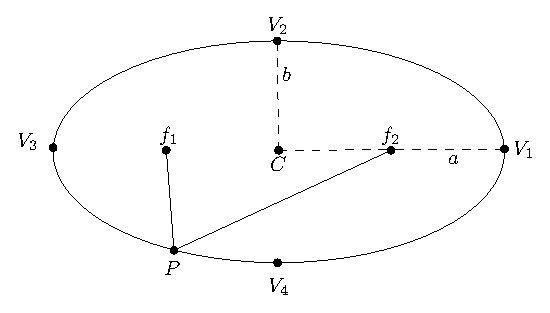
\includegraphics[scale=.8]{images/ellipse_focalDef.eps}
	\caption{Ellipse mit Brennpunkten $f_1, f_2$, Zentrum $C$, Hauptachse $a$, Nebenachse $b$ und Scheitelpunkten $V_1$ und $V_2$}
	\label{fig:ellipseDef}
\end{figure}

In ihrer einfachsten Form liegt die Ellipse im Zentrum des Koordinatensystems und ihre Haupt- und Nebenachse $a$ und $b$ sind achsenausgerichtet. Das heißt ihre Hauptachse liegt auf der $X$-Achse und ihre Nebenachse auf der $Y$-Achse. Sie kann dann in der impliziten Form

\begin{equation} \label{eq:ellipseNoRotNoTrans}
\frac{x^2}{a^2} + \frac{y^2}{b^2} = 1
\end{equation} 

beschrieben werden.

\begin{figure}[!htb]
	\centering
	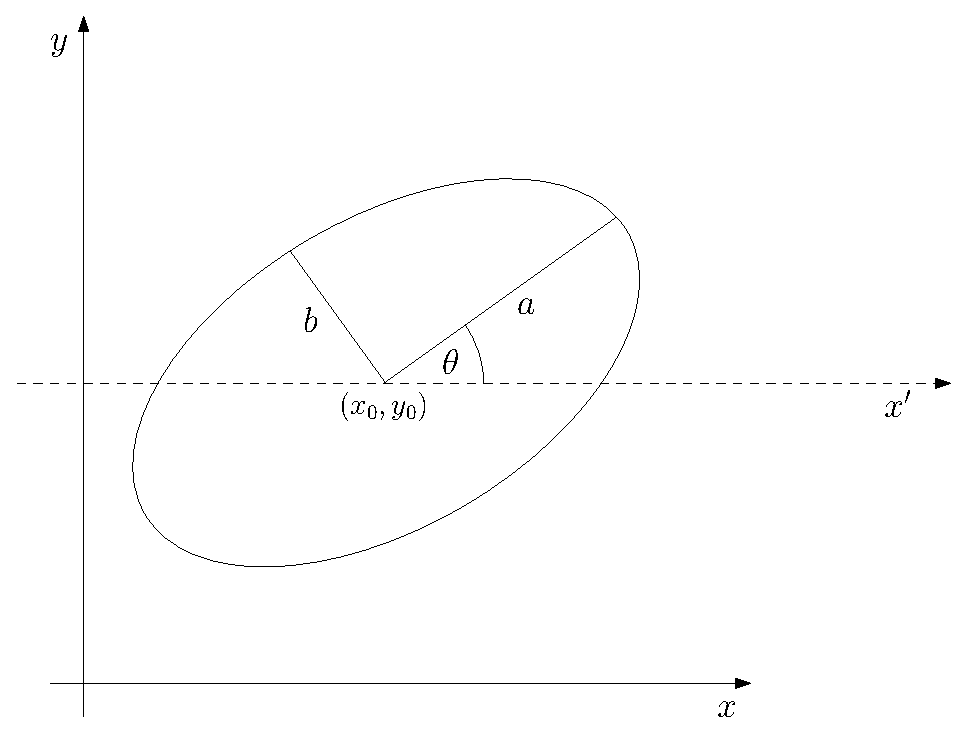
\includegraphics[scale=.7]{images/ellipse.eps}
	\caption{Ellipse mit Zentrum $(x_0, y_0)$, Hauptachse $a$, Nebenachse $b$, sowie Drehwinkel $\theta$}
	\label{fig:ellipse}
\end{figure}

Befindet sich die Ellipse nicht im Ursprung so muss eine Verschiebung beziehungsweise bei einer Rotation ein Drehwinkel (siehe Abbildung \ref{fig:ellipse}) ergänzt werden. 

\begin{equation} \label{eq:ellipseNoRotTrans}
\frac{\left(x-x_0\right)^2}{a^2} + \frac{\left(y-y_0\right)^2}{b^2} = 1
\end{equation} 

\begin{equation} \label{eq:ellipseRotTrans}
\frac{((x - x_0)\cos\theta + (y - y_0)\sin\theta)^2}{a^2} + \frac{((x - x_0)\sin\theta - (y - y_0)\cos\theta)^2}{b^2} = 1
\end{equation} 

mit Ellipsenzentrum $(x_0,y_0)\in\mathbb{R}^2$, Hauptachsen $a,b\in\mathbb{R}^+$, sowie Drehwinkel $\theta \in [0,2\pi)$ oder parametrisiert

\begin{equation} \label{eq:ellipseRotTransParam}
\begin{pmatrix}x \\ y\end{pmatrix} = \begin{pmatrix}x_0 + a\cos\phi\cos\theta - b\sin\phi\sin\theta \\ 
y_0 + a\cos\phi\sin\theta + b\sin\phi\cos\theta\end{pmatrix}
\end{equation}
mit $\phi \in [0, 2\pi)$ und $x_0, y_0, a,b, \theta$ wie oben.

In ihrer allgemeinsten Form lässt sich eine Ellipse durch ein implizites Polynom zweiten Grades charakterisieren
\begin{equation} \label{eq:ellipseQuadratic}
ax^2 + by^2 + cxy + dx + ey + f = 0 \quad \text{mit}\quad c^2-4ab < 0
\end{equation} 
mit $a,b,c,d,e,f \in \mathbb{R}$. Eine Ellipse lässt sich also durch sechs Punkte eindeutig beschrieben (fünf, wenn man $f$ auf eins skaliert).


Die beiden Formen \ref{eq:ellipseRotTrans} und \ref{eq:ellipseQuadratic} sind äquivalent, falls die Ellipse nicht degeneriert ist (ohne Beweis) \cite{Lawrence1972}. Da wir die Umformung von \ref{eq:ellipseRotTrans} nach \ref{eq:ellipseQuadratic} später brauchen, wird sie hier einmal exemplarisch vorgeführt. 

Zunächst einmal fällt auf, dass der gemischte Term $cxy$ genau dann null ist, wenn die Ellipse nicht rotiert wurde. Im ersten Schritt versuchen wir also die Rotation der Ellipse rückgängig zu machen, um den Rotationswinkel bestimmen zu können.

Die Gleichung \ref{eq:ellipseQuadratic} kann umgeformt werden zu:
\begin{equation*}
\begin{aligned}
\underbrace{\begin{pmatrix}x & y\end{pmatrix}}_{=:u^T}\underbrace{\begin{pmatrix}a & \frac{c}{2} \\ \frac{c}{2} & b\end{pmatrix}}_{=: M}\underbrace{\begin{pmatrix}x \\ y\end{pmatrix}}_{=u} +\begin{pmatrix}d & e\end{pmatrix}\underbrace{\begin{pmatrix}x \\ y\end{pmatrix}}_{=u}+ f = 0 \\
\Leftrightarrow u^TMu +\begin{pmatrix}d & e\end{pmatrix}u + f = 0 \\
\end{aligned}
\end{equation*} 
Der gemischte Term wird alleine durch $M = \begin{pmatrix}a & \frac{c}{2} \\ \frac{c}{2} & b\end{pmatrix}$ bestimmt. Da die Matrix $M$ symmetrisch ist, ist sie orthogonal diagonalisierbar. Des Weiteren hat $M$ zwei von null verschiedene Eigenwerte, denn 
\[
\det M = ab - \dfrac{c^2}{4}
\] ist nur dann gleich null, wenn $c^2 - 4ab = 0$, was ein Widerspruch zur Annahme in \ref{eq:ellipseQuadratic} ist. $M$ hat somit eine von null verschiedene Determinante und somit vollen Rang, hat also zwei von null verschiedene Eigenwerte. Insbesondere gibt es also zwei Eigenvektoren von $M$, die zueinander orthogonal sind.

Es gilt $M = S^TDS$, wobei $S\in\mathbb{R}^{2\times2}$ eine orthogonale Matrix mit den normierten Eigenvektoren als Zeilen und $D = \text{diag}(\lambda_1, \lambda_2)\in\mathbb{R}^{2\times2}$ eine Diagonalmatrix mit den beiden Eigenwerten von $M$ auf der Diagonalen ist. Ohne Beschränkung der Allgemeinheit gelte $\lambda_1 <= \lambda_2$, andernfalls vertausche die Eigenvektoren in $S$. 

Sei nun $v := Su$.
So gilt:

\begin{equation} \label{eq:PCARot}
\begin{aligned}
&u^T(S^TDS)u +\begin{pmatrix}d & e\end{pmatrix}\underbrace{(S^TS)}_{=\ind}u + f = 0 \\
\Leftrightarrow\quad &(Su)^TD(Su) +\begin{pmatrix}d & e\end{pmatrix}S^T(Su) + f = 0 \\
\Leftrightarrow\quad &v^{T}Dv +\begin{pmatrix}d & e\end{pmatrix}S^Tv + f = 0 
\end{aligned}
\end{equation}

Man kann leicht nachrechnen, dass der gemischte Teil somit eliminiert wurde. Durch Anwenden der Transformation $S$ wurde $u$ also in das Koordinatensystem, in dem die Ellipse achsenausgerichtet ist,  transformiert.

Eine Rotationsmatrix mit Rotationswinkel $\theta$ ist definiert durch: 
\begin{equation}
\begin{aligned}
R = \begin{pmatrix}\cos\theta & -\sin\theta \\ \sin\theta & \cos\theta\end{pmatrix}
\end{aligned}
\end{equation}

Es gilt offenbar $S = R$ für ein geeignetes $\theta$, da die Eigenvektoren normiert und orthogonal zueinander sind. $\theta$ kann also einfach ausgerechnet werden, denn es gilt:

\begin{equation*}
\theta = \atant(\sin\theta, \cos\theta) = \atant(S_{2,1}, S_{1,1})
\end{equation*}

Multipliziert man nun \ref{eq:PCARot} aus ergibt sich:

\begin{equation}\label{eq:ellipseCenter}
\begin{aligned}
&\lambda_1v_1^2 + \lambda_2v_2^2 + \underbrace{\begin{pmatrix}d & e\end{pmatrix}S^T}_{=:(d', e')}v + f = 0 \\
\Leftrightarrow\quad &\lambda_1v_1^2 + \lambda_2v_2^2 + d'v_1 + e'v_2 + f = 0 \\
\Leftrightarrow\quad &(\lambda_1v_1^2 + d'v_1)+ (\lambda_2v_2^2 + e'v_2) + f = 0\\
\Leftrightarrow\quad &(\lambda_1v_1^2 + d'v_1) + (\frac{d'^2}{4\lambda_1} - \frac{d'^2}{4\lambda_1}) + (\lambda_2v_2^2 + e'v_2) + (\frac{e'^2}{4\lambda_2} - \frac{e'^2}{4\lambda_2}) + f = 0 \\
\Leftrightarrow\quad &\left[\lambda_1\left(v_1^2 + \frac{2d'}{2\lambda_1}v_1 + \frac{d'^2}{4\lambda_1^2}\right) - \frac{d'^2}{4\lambda_1}\right] +\left[\lambda_2\left(v_2^2 + \frac{2e'}{2\lambda_2}v_2 + \frac{e'^2}{4\lambda_2^2}\right) - \frac{e'^2}{4\lambda_2}\right] + f = 0 \\
\Leftrightarrow\quad &\lambda_1(v_1 + \underbrace{\frac{d'}{2\lambda_1}v_1}_{ = -x'_0})^2 +\lambda_2(v_2 + \underbrace{\frac{e'}{2\lambda_2}v_2}_{ = -y'_0})^2 - \underbrace{(\frac{d'^2}{4\lambda_1} + \frac{e'^2}{4\lambda_2} - f)}_{=:\sigma} = 0,
\end{aligned}
\end{equation}

da $\lambda_1, \lambda_2 \neq 0$. 

Das Zentrum der transformierten Ellipse kann nun aus \ref{eq:ellipseCenter} einfach abgelesen werden. Um das Zentrum der eigentlichen Ellipse zu bestimmen, muss mit der inversen Rotation $S^T$ multipliziert werden:
\begin{equation*}
(x_0, y_0)^T = S^T(x'_0, y'_0)^T
\end{equation*}

Obige Gleichung lässt sich anschließend weiter vereinfachen: 


\begin{equation} \label{eq:PCAKoeff}
\begin{aligned}
&\lambda_1(v_1 -x'_0)^2 +\lambda_2(v_2 -y'_0)^2 = \sigma \\
\Leftrightarrow\quad & \frac{\lambda_1}{\sigma}(v_1 -x'_0)^2 +\frac{\lambda_2}{\sigma}(v_2 -y'_0)^2  =1
\end{aligned}
\end{equation}

wobei $\sigma \neq 0$, wenn die Ellipse nicht zum Punkt entartet ist \cite{Lawrence1972}. Vergleicht man nun \ref{eq:PCAKoeff} mit \ref{eq:ellipseNoRotTrans} so sieht man das

\begin{equation}
\begin{aligned}
&\frac{\lambda_1}{\sigma} = \frac{1}{a^2} &\text{und}\quad &\frac{\lambda_2}{\sigma} = \frac{1}{b^2}\\
\Leftrightarrow\quad & \sqrt{\frac{\sigma}{\lambda_1}}  = a  &\text{und}\quad & \sqrt{\frac{\sigma}{\lambda_2}}  = b
\end{aligned}
\end{equation}

Es gilt wie erwartet $a \geq b$, da $\lambda_1 \leq \lambda_2$


\subsection{Abstand: Punkt zu Ellipse}
\label{sc:distPointEllipse}
Das hier beschriebene Verfahren zur Bestimmung der kürzesten euklidischen Distanz eines Punktes zu einer Ellipse stammt aus der Arbeit von David Eberly \cite{Eberly2013}.
Wir betrachten nur Ellipsen im Ursprung, die achsenausgerichtet sind und darüber hinaus nur Punkte im ersten Quadranten. Ansonsten wir die Ellipse in den Ursprung verschoben und um ihren entgegengesetzten Drehwinkel rotiert. Da die Ellipse dann bezüglich der $X$- und $Y$- Achse symmetrisch ist, kann der Punkt einfach durch Spiegelung in den richtigen Quadranten transformiert werden. Der Abstand ändert sich dadurch nicht. 

Wir bezeichnen von nun an $Q = (y_0, y_1)$ als eine Punkt, dessen Distanz zur Ellipse wir berechnen wollen und $E = (x_0, x_1)$ als denjenigen eindeutigen Punkt, welcher auf der Ellipse liegt und die kürzeste euklidische Distanz vom Punkt $Q$ hat. 

Aufgrund dieser Forderungen können wir ohne Beschränkung der Allgemeinheit folgende Aussagen treffen:
\begin{itemize}
	\item Die Ellipse kann stets durch die implizite Gleichung 
	\begin{equation}\label{eq:distEqParam} \frac{x_0^2}{a^2} + \frac{x_1^2}{b^2} = 1\end{equation}
	 mit $a \geq b \geq 0$ beziehungsweise
	in der parametrischen Form \[\mathcal{E}(\theta) = (a\cos\phi, b\sin\phi)  \tag*{$\phi \in [0, 2\pi)$}\] beschrieben werden.
	\item Es gilt $y_0,y_1,x_0, x_1 \geq 0$
\end{itemize}

Für die quadrierte Distanz von einem beliebigen Punkt $Q$ zu einem Punkt $\mathcal{E}(\theta)$ auf der Ellipse gilt dann
\begin{equation}
	F(\theta) = \abs{\mathcal{E}(\theta) - Q}^2.
\end{equation}

Die Ableitung von $F$
\begin{equation}
F'(\theta) = 2\left(\mathcal{E}(\theta) - Q\right) \cdot \mathcal{E}'(\theta).
\end{equation}

wird null, wenn $\left(\mathcal{E}(\theta) - Q\right)$ und $ \mathcal{E}'(\theta)$ zu einander orthogonal sind. Daraus folgt, dass der Vektor von $Q$ zu $E$ senkrecht zur Ellipse stehen muss.  (siehe Abbildung \ref{fig:ellipseDist}). 


\begin{figure}[!htb]
	\centering
	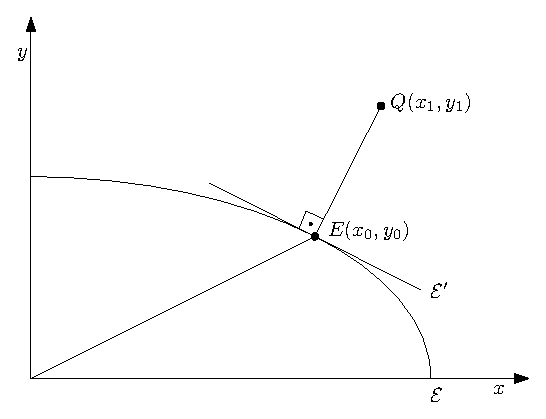
\includegraphics[scale=.9]{images/ellipseQuery.eps}
	\caption{Ellipsenausschnitt im ersten Quadranten mit Abfragepunkt $Q$ und eingezeichneter kürzester Distanz zur Ellipse}
	\label{fig:ellipseDist}
\end{figure}

Betrachten wir also die Funktion:
\begin{equation} \label{eq:ellipseDistEq}
	G(x_0,x_1) = \frac{x_0^2}{a^2} + \frac{x_1^2}{b^2} - 1.
\end{equation}
$(x_0,x_1)$ ist genau dann ein Punkt auf der Ellipse, wenn $G(x_0,x_1) = 0$. Der Gradient von $G$ in $(x_0,x_1)$ ist ein Normalenvektor auf der Ellipse, somit auch der halbe Gradient $\nabla G(x_0,x_1)/2$. Der Vektor von $E$ zu $Q$ muss dieselbe Richtung haben. Es gilt somit:

\begin{equation}
	(y_0,y_1) - (x_0, x_1) = t\frac{\nabla G(x_0,x_1)}{2} = t\left(\frac{x_0}{a^2},\frac{x_1}{b^2}\right)
\end{equation}
für ein $t\in\mathbb{R}$.

Umgestellt nach $y_0$ und $y_1$, beziehungsweise nach $x_0$ und $x_1$ ergibt sich:

\begin{equation}\label{eq:ellipseDistY}
y_0 = x_0\left(1 + \frac{t}{a^2}\right), \quad y_1 = x_1\left(1 + \frac{t}{b^2}\right)
\end{equation}

\begin{equation}\label{eq:ellipseDistX}
x_0 = \frac{a^2y_0}{t+a^2},\quad x_1 = \frac{b^2y_1}{t+b^2}
\end{equation}


\bigskip
Man macht nun eine Fallunterscheidung:

\begin{enumerate}
	\item Der einfachste Fall ist, wenn sich der Punkt $Q$ auf der $Y$-Achse (außer $(0,0)$) befindet, wenn also gilt $y_0 = 0, y_1 > 0$.
	Da die Hauptachse nach der $X$-Achse ausgerichtet ist und $a >= b$ gilt, ist der Punkt auf der Ellipse mit der kürzesten Distanz zu $Q$ offenbar $E = (0, b)$ und für die Distanz gilt $d = \abs{y_1 - b}$.
	\item Als nächstes betrachten wir ein $Q$ auf der $X$-Achse (einschließlich $(0,0)$), wenn also gilt  $y_0 \geq 0, y_1 = 0$. Es gilt also mit \ref{eq:ellipseDistY}
	\[
		y_0 = x_0\left(1 + \frac{t}{a^2}\right), \quad 0 = x_1\left(1 + \frac{t}{b^2}\right)
	\]
	
	Wenn $x_1 = 0$ gilt, muss $x_0 = a$ gelten, damit $E(x_0,x_1)$ auf der Ellipse ist. Es  gilt analog zum ersten Fall $E=(a,0)$ mit $d = \abs{y_0 - a}$ 
	
	Gilt $x_1 \neq 0$, so können wir in der zweiten Gleichung durch $x_1$ teilen und es folgt $t = -b^2$ und somit $y_0 = x_0\left(1 - \frac{b^2}{a^2}\right)$. Auf Grund der Krümmung der Ellipse gilt außerdem $x_0 < a$ und somit ergibt sich zusammen mit \ref{eq:ellipseDistX} die Ungleichung:
	\begin{equation*}
	\begin{aligned}
		&x_0 = \frac{a^2y_0}{a^2 - b^2} < a \\
		\Leftrightarrow\quad &y_0 < \frac{a^2 - b^2}{a} < a
	\end{aligned}
	\end{equation*}
		
	Für Punkte $Q(y_0,0)$ mit $y_0 \geq \frac{a^2 - b^2}{a}$, ist der kürzeste Punkt also wieder $E(a,0)$
	
	Für Punkte $Q(y_0,0)$ mit $y_0 < \frac{a^2 - b^2}{a}$, muss für $E(x_0,x_1)$ nach Umstellen der Ellipsengleichung \ref{eq:distEqParam}\quad$x_1 = b\cdot\sqrt{1-\left(\frac{x_0}{a}\right)}$ gelten. 
	Die Distanz beträgt dann:

	\[
		d^2 = (x_0 - y_0)^2 + x_1^2 = b^2\left(1 - \frac{y_0^2}{a^2 - b^2}\right)
	\]
	\item Der letzte Fall, den wir betrachten müssen, ist der allgemeinste Fall. Es gilt $y_0 > 0$, sowie $y_1 > 0$. Da wir uns nur im ersten Quadranten bewegen, gilt darüber hinaus $x_0, x_1 \geq 0$. Mit diesen Eigenschaften und \ref{eq:ellipseDistY} lässt sich folgende Einschränkung für $t$ herleiten:
	\begin{equation}
	\begin{aligned}
	& 0 < y_0 = x_0\left(1 + \frac{t}{a^2}\right)\\
	\Leftrightarrow\quad& -1\cdot a^2 < t.
	\end{aligned}
	\end{equation}
	Analog ergibt sich mit $y_1\colon -b^2 < t$. Da $a\geq b$ gilt, reicht es, sich nur die zweite Ungleichung anzuschauen, da sie die erste impliziert. Setzt man nun \ref{eq:ellipseDistX} in \ref{eq:ellipseDistEq} ein, erhält man:
	
	\begin{equation}
		F(t) = \left(\frac{ay_0}{t+a^2}\right)^2 + \left(\frac{by_1}{t+b^2}\right)^2 - 1
	\end{equation}
	
	Man kann nun zeigen, dass diese Funktion auf dem gesamten Intervall $[-b^2,\infty)$ monoton fällt und links gekrümmt ist. Darüber hinaus gilt:
	\[
	\lim\limits_{t \searrow -b^2}{F(t)}	= +\infty, \quad\lim\limits_{t \rightarrow \infty}{F(t)}	= 1.
	\]
	Da $F$ stetig ist, muss es also eine Nullstelle geben, die aufgrund des Monotonie- und Krümmungsverhaltens sogar eindeutig ist. Die Nullstelle lässt sich beispielsweise durch Intervallschachtelung oder Newton-Verfahren bestimmen. 
\end{enumerate}









